%----------------------------------------------------------------------------------------
% DE CORRELATIECOËFFICIËNT. Alle opgaven zijn eigen werk; alle gegevens zijn verzonnen.
%
% Opbouw: Probleem, Start, leerstof, en op een nieuwe pagina de Opdrachten en Test jezelf (geen Koppel in de 2de graad).
% Labels van dit hoofdstuk beginnen met h2-.
% Leerlingen berekenen r met ICT; de definitie van r hoort niet bij het leerplandoel (ook niet in B+S''), dus geen formule.
% Verschil per pakket: een opdracht over een omgekeerd evenredig verband (f(x) = c/x, pakket 3-5: in B+ is c/x een keuzedeel).
% Nagerekend: alle r-waarden en regressielijnen met Python (numpy.corrcoef en kleinste kwadraten).
%----------------------------------------------------------------------------------------

\mychapter{2}{De correlatiecoëfficiënt}

\begin{probleem}
Tijdens een stage in een basisschool laat Mila twaalf kinderen van 6 tot 12 jaar een leestest maken (score op 50). Voor de turnles noteert ze ook hun schoenmaat. (De gegevens zijn verzonnen.)

\vspace{1mm}
{\centering\kleinetabel[schoenmaat][score]{12}{28 & 29 & 30 & 31 & 31 & 33 & 33 & 34 & 35 & 36 & 37 & 38}{12 & 15 & 18 & 16 & 24 & 22 & 28 & 30 & 33 & 31 & 38 & 42}\par}

\vspace{1mm}
Mila ziet het meteen: kinderen met grotere voeten lezen beter. Hoe sterk is dat verband? Kun je die sterkte in één getal uitdrukken? En moet een kind dat slecht leest dan grotere schoenen krijgen?
\end{probleem}

\lkr{Leerplan \pakketnaam: LPD \alleenvoor{2}{34}\alleenvoor{3}{36}\alleenvoor{4,5}{40} (dit hoofdstuk: de correlatiecoëfficiënt met ICT berekenen en interpreteren, sterkte en richting, de grenzen van $r$ (alleen lineair, gevoelig voor uitschieters, zegt niets over de steilheid) en het verschil tussen correlatie en oorzakelijk verband). Leerlingen berekenen $r$ niet met de hand maar met ICT: het leerplan vraagt $r$ te bepalen en te interpreteren, niet de definitie te bestuderen. Het leerplan stelt voor het doel te laten terugkeren bij de functies: hier gebeurt dat met de remweg (tweedegraads, hoofdstuk 1) en de opgegooide bal (parabool)\alleenvoor{3,4,5}{, en met een fietstocht waarbij de rijtijd omgekeerd evenredig is met de snelheid ($f(x) = c/x$)}. De grenzen voor sterk, matig en zwak zijn een afspraak van dit boek; gebruikt uw school andere grenzen, vermeld dat dan. Bij het probleem lachen de meeste leerlingen om de vraag over de schoenen, maar laat ze de echte verklaring (de leeftijd) zelf zoeken.}

In het vorige hoofdstuk beschreef je de sterkte van een verband met woorden: sterk of zwak, naargelang de punten dicht bij een rechte liggen of niet. Maar wanneer is een verband ``sterk''? Twee mensen kunnen daar anders over oordelen. In dit hoofdstuk leer je een getal kennen dat de sterkte en de richting van een lineair verband meet: de \textit{correlatiecoëfficiënt}. Je berekent het met ICT, net als de regressielijn. Daarna zie je wat dat getal niet zegt, en waarom een sterk verband nog niet betekent dat het ene het andere veroorzaakt.

\begin{oefeningen}[Start]
\oef{h2-start-1}

\needspace{16\baselineskip}
\oef{h2-verken}
\end{oefeningen}

%========================================================================================
\section{Hoe sterk is een verband?}

\subsection{Een getal voor de sterkte en de richting}

Hoe meet je met een getal of een puntenwolk stijgt of daalt? Neem de ijsjes uit het vorige hoofdstuk, met het gemiddelde punt $(24, 160)$. Trek door dat punt een verticale en een horizontale lijn. Zo verdeel je het diagram in vier kwadranten.

\naast{Rechtsboven liggen de dagen die warmer waren dan gemiddeld \textit{en} meer ijsjes verkochten dan gemiddeld. Linksonder liggen de dagen die kouder waren \textit{en} minder verkochten. Bij een positief verband liggen bijna alle punten in die twee kwadranten: hier acht van de tien. Linksboven ligt er één, en één ligt op de lijn.

\vspace{1mm}
Bij een negatief verband is het omgekeerd: de meeste punten liggen linksboven en rechtsonder. En als er geen verband is, liggen de punten ongeveer gelijk verspreid over de vier kwadranten.}{\begin{tikzpicture}[x=.27cm,y=.016cm,font=\scriptsize]
  \diagram[$T$ (°C)][$N$ (ijsjes)]{14}{2}{34}{0}{20}{280}
  \xas{14,18,...,34}\yas{0,40,...,280}
  \gemlijnen{24}{160}{14}{34}{0}{280}
  \punten{(17,85) (19,89) (20,125) (22,120) (23,165) (24,145) (26,180) (28,225) (30,221) (31,245)}
  \gempunt{24}{160}
  \node[font=\large,text=inkt] at (32.5,262) {$+$};
  \node[font=\large,text=inkt] at (15.5,20) {$+$};
  \node[font=\large,text=inkt] at (15.5,262) {$-$};
  \node[font=\large,text=inkt] at (32.5,20) {$-$};
\end{tikzpicture}}

Waarom de tekens $+$ en $-$ in de figuur? Rechtsboven is $x - \xbar > 0$ en $y - \ybar > 0$, dus het product $(x - \xbar)(y - \ybar)$ is positief. Linksonder zijn beide factoren negatief, en is het product ook positief. In de twee andere kwadranten is het product negatief. ICT telt die producten op voor alle punten, en deelt de som door een getal dat ervoor zorgt dat de uitkomst altijd tussen $-1$ en $1$ ligt. Zo ontstaat één getal.

\begin{theorie}
De \textbf{\textcolor{accent}{correlatiecoëfficiënt}} $r$ meet de sterkte en de richting van het lineaire verband tussen twee variabelen. Altijd geldt

\vspace{1mm}
\qquad $\formule{-1 \leqslant r \leqslant 1}$

\vspace{1mm}
Bij een positief verband is $\formule{r > 0}$, bij een negatief verband $\formule{r < 0}$. Hoe dichter $r$ bij $1$ of $-1$ ligt, hoe sterker het lineaire verband. Liggen alle punten op één rechte, dan is $\formule{r = 1}$ (stijgend) of $\formule{r = -1}$ (dalend).
\end{theorie}

De figuren tonen puntenwolken met hun correlatiecoëfficiënt. Van links naar rechts liggen de punten steeds minder dicht bij een stijgende rechte, tot ze bij $r = 0$ geen richting meer hebben. Daarna dalen ze, steeds duidelijker.

\figuren{\begin{tikzpicture}[x=.2cm,y=.2cm,font=\scriptsize]
  \diagram[][]{0}{2}{10}{0}{2}{10}
  \punten{(1,1.3) (2,2.1) (3,2.9) (4,3.7) (5,4.5) (6,5.3) (7,6.1) (8,6.9) (9,7.7)}
  \node[below] at (5,-.6) {$r = 1$};
\end{tikzpicture}\hfill
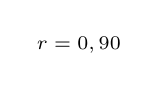
\begin{tikzpicture}[x=.2cm,y=.2cm,font=\scriptsize]
  \diagram[][]{0}{2}{10}{0}{2}{10}
  \punten{(1.2,1.6) (2.1,2.9) (2.2,3.5) (2.5,4.8) (3.4,4.9) (3.4,3.9) (3.8,4.4) (4.2,5.2) (5.9,4.9) (6.4,6.2) (6.5,7.2) (8.3,6.7) (8.4,6.9) (8.6,6.8)}
  \node[below] at (5,-.6) {$r = 0,90$};
\end{tikzpicture}\hfill
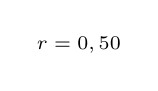
\begin{tikzpicture}[x=.2cm,y=.2cm,font=\scriptsize]
  \diagram[][]{0}{2}{10}{0}{2}{10}
  \punten{(0.9,3.9) (1.5,4.2) (1.7,5.7) (2.7,4.5) (3.8,3.2) (4.1,5.8) (4.3,1.5) (4.5,6.7) (4.5,4.4) (4.7,3.5) (4.7,6.2) (6.4,7.1) (6.9,6.2) (8.8,7.3)}
  \node[below] at (5,-.6) {$r = 0,50$};
\end{tikzpicture}\hfill
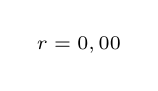
\begin{tikzpicture}[x=.2cm,y=.2cm,font=\scriptsize]
  \diagram[][]{0}{2}{10}{0}{2}{10}
  \punten{(1.5,4.3) (1.6,4.3) (2.2,3.1) (2.2,7.3) (3.2,7.1) (3.6,4.9) (3.8,4.8) (4,5.6) (4.6,3.1) (5.6,7) (7.6,3.6) (8.4,2.5) (9.1,5.2) (9.2,7.3)}
  \node[below] at (5,-.6) {$r = 0,00$};
\end{tikzpicture}\hfill
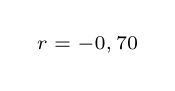
\begin{tikzpicture}[x=.2cm,y=.2cm,font=\scriptsize]
  \diagram[][]{0}{2}{10}{0}{2}{10}
  \punten{(1.6,6) (1.8,6.8) (2.5,6.9) (3,6.1) (5.5,6.8) (5.5,5.5) (5.6,5.1) (5.9,4.4) (7.6,2.6) (7.7,4.5) (8,2.8) (8.2,6.6) (8.8,4.1) (8.9,1.9)}
  \node[below] at (5,-.6) {$r = -0,70$};
\end{tikzpicture}\hfill
\begin{tikzpicture}[x=.2cm,y=.2cm,font=\scriptsize]
  \diagram[][]{0}{2}{10}{0}{2}{10}
  \punten{(1,8.7) (2,7.9) (3,7.1) (4,6.3) (5,5.5) (6,4.7) (7,3.9) (8,3.1) (9,2.3)}
  \node[below] at (5,-.6) {$r = -1$};
\end{tikzpicture}}

Let op: $r = 0$ betekent niet dat de punten op een horizontale rechte liggen. Het betekent dat er geen lineair verband is: de wolk stijgt noch daalt.

\voorbeeld{}{Het spreidingsdiagram toont voor zestien gemeenten de afstand $x$ tot de dichtstbijzijnde stad (in km) en de gemiddelde prijs $y$ van een bouwgrond (in euro per m²). Is $r$ positief of negatief? Ligt $r$ dicht bij $0$ of bij $\pm 1$?\label{vb:h2-kwadrant}}{%
\naast{\uitleg{We tekenen in gedachten de lijnen door het gemiddelde punt (het vierkantje), en kijken in welke kwadranten de punten liggen.}
\begin{stappenvrij}{1.6cm}{5.9cm}
\text{teken} & De meeste punten liggen linksboven en rechtsonder: daar is het product negatief. Dus $r < 0$. \\
\text{sterkte} & De punten liggen vrij dicht bij een dalende rechte, maar niet erop: $r$ ligt dicht bij $-1$, bijvoorbeeld rond $-0,9$.
\end{stappenvrij}
\vspace{1mm}
ICT geeft hier $r = -0,98$: een sterk negatief verband. Verder van de stad is bouwgrond goedkoper.}{\begin{tikzpicture}[x=.13cm,y=.016cm,font=\scriptsize]
  \diagram[$x$ (km)][$y$ (euro/m²)]{0}{5}{40}{100}{25}{400}
  \xas{0,10,...,40}\yas{100,200,300,400}
  \gemlijnen{17.1875}{260.625}{0}{40}{100}{400}
  \punten{(2,380) (3,345) (5,350) (6,310) (8,325) (10,300) (12,270) (14,290) (17,250) (20,240) (22,215) (25,200) (28,215) (31,170) (34,160) (38,150)}
  \gempunt{17.1875}{260.625}
\end{tikzpicture}}}

\begin{oefeningen}
\needspace{16\baselineskip}
\oef{h2-kwadrant}
\end{oefeningen}

\subsection{Sterk of zwak?}

Een getal tussen $-1$ en $1$ is handig, maar wanneer noem je een verband sterk? Daarvoor bestaat geen natuurwet, wel een afspraak. Je kijkt naar $\abs{r}$, de waarde van $r$ zonder het teken: het teken zegt de richting, $\abs{r}$ de sterkte.

\begin{theorie}
De sterkte van een lineair verband hangt af van $\abs{r}$:

\vspace{1mm}
{\centering\renewcommand{\arraystretch}{1.35}\begin{tabular}{|c|c|c|}\hline
$\formule{0,8 \leqslant \abs{r} \leqslant 1}$ & $\formule{0,5 \leqslant \abs{r} < 0,8}$ & $\formule{\abs{r} < 0,5}$ \\ \hline
\textbf{\textcolor{accent}{sterk}} verband & \textbf{\textcolor{accent}{matig}} verband & \textbf{\textcolor{accent}{zwak}} of geen verband \\ \hline
\end{tabular}\par}
\end{theorie}

Dat is een afspraak van dit boek: andere boeken en onderzoekers leggen de grenzen iets anders. Belangrijk is dat $r = -0,9$ een sterker verband geeft dan $r = 0,6$. Het minteken zegt alleen dat de wolk daalt.

\voorbeeld{}{In een onderzoek bij leerlingen van het vierde jaar is de correlatiecoëfficiënt tussen het aantal uren schermtijd per dag en het aantal uren slaap per nacht $r = -0,62$. Wat betekent dat?\label{vb:h2-sterkte}}{%
\uitleg{Het teken zegt de richting, $\abs{r}$ de sterkte.}
\begin{stappen}
r < 0 & Een negatief verband: wie meer schermtijd heeft, slaapt meestal minder. \\
\abs{r} = 0,62 & Tussen 0,5 en 0,8: een matig verband.
\end{stappen}
Er zijn dus veel leerlingen die er niet in passen: met veel schermtijd en toch lang slapen, of omgekeerd. De punten liggen niet dicht bij een rechte.}

\begin{oefeningen}
\oef{h2-sterkte}
\end{oefeningen}

Met wat oefening kun je $r$ ook schatten uit een spreidingsdiagram. Kijk eerst naar de richting (het teken), dan naar hoe dicht de punten bij een rechte liggen.

\voorbeeld{}{Welke van de waarden $0,98$, $0,75$ en $-0,40$ hoort bij welk spreidingsdiagram?\label{vb:h2-schatten}}{%
\figuren{\begin{tikzpicture}[x=.25cm,y=.25cm,font=\scriptsize]
  \diagram[][]{0}{2}{10}{0}{2}{10}
  \punten{(1.7,4.8) (1.9,2.7) (2.9,3.8) (3.2,3.5) (3.8,1.8) (4.2,4.7) (4.8,5.7) (5.2,5.5) (5.6,5.9) (5.9,5.1) (6.3,6.6) (6.3,5) (6.7,6.8) (6.9,8)}
  \node[below,font=\small\bfseries] at (5,-.6) {A};
\end{tikzpicture}\qquad\qquad
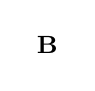
\begin{tikzpicture}[x=.25cm,y=.25cm,font=\scriptsize]
  \diagram[][]{0}{2}{10}{0}{2}{10}
  \punten{(1.1,5) (1.2,4.7) (1.5,7.4) (2,2.7) (2,6.1) (2.5,6.6) (4,6.1) (4.1,7.1) (4.9,4.2) (6.5,5.1) (7.5,1.8) (8.3,4.8) (9.2,3.1) (9.2,5.3)}
  \node[below,font=\small\bfseries] at (5,-.6) {B};
\end{tikzpicture}\qquad\qquad
\begin{tikzpicture}[x=.25cm,y=.25cm,font=\scriptsize]
  \diagram[][]{0}{2}{10}{0}{2}{10}
  \punten{(1.5,1.6) (2.4,2.7) (3.4,2.9) (4.7,4.1) (5.2,4.1) (5.4,5) (5.7,4.7) (6.3,5.6) (6.9,6) (7.3,6) (7.6,6.3) (7.6,6.4) (8.4,7.2) (8.8,7.4)}
  \node[below,font=\small\bfseries] at (5,-.6) {C};
\end{tikzpicture}}
\uitleg{Eerst het teken, dan de sterkte.}
\begin{stappen}
\text{B: } r = -0,40 & De enige wolk die (een beetje) daalt. De punten liggen ver uit elkaar: zwak. \\
\text{C: } r = 0,98 & Stijgend, en de punten liggen bijna op een rechte. \\
\text{A: } r = 0,75 & Stijgend, maar de punten liggen verder van een rechte dan bij C.
\end{stappen}}

\begin{oefeningen}
\needspace{16\baselineskip}
\oef{h2-schatten}
\end{oefeningen}

Een veelgemaakte fout: denken dat $r$ zegt hoe \textit{steil} de wolk is. Dat is niet zo. De twee wolken hieronder hebben precies dezelfde $r = 0,98$: de punten liggen even dicht bij hun rechte. Maar de linkse regressielijn heeft rico $1,93$ en de rechtse rico $0,48$. De steilheid lees je af aan de rico van de regressielijn, de sterkte aan $r$.

\figuren{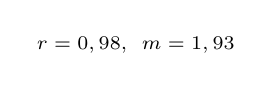
\begin{tikzpicture}[x=.4cm,y=.18cm,font=\scriptsize]
  \diagram{0}{1}{9}{0}{2}{18}
  \xas{0,2,...,8}\yas{0,6,12,18}
  \rechte{0.5}{8.8}{1.9333}{1.3}
  \punten{(1,3.8) (2,3.8) (3,8) (4,8.6) (5,12.2) (6,12) (7,14.4) (8,17.2)}
  \node[below=5mm] at (4.5,0) {$r = 0,98$, \ $m = 1,93$};
\end{tikzpicture}\qquad\qquad
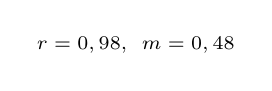
\begin{tikzpicture}[x=.4cm,y=.18cm,font=\scriptsize]
  \diagram{0}{1}{9}{0}{2}{18}
  \xas{0,2,...,8}\yas{0,6,12,18}
  \rechte{0.5}{8.8}{0.4833}{3.075}
  \punten{(1,3.7) (2,3.7) (3,4.75) (4,4.9) (5,5.8) (6,5.75) (7,6.35) (8,7.05)}
  \node[below=5mm] at (4.5,0) {$r = 0,98$, \ $m = 0,48$};
\end{tikzpicture}}

%========================================================================================
\section{De correlatiecoëfficiënt met ICT}

Met de hand rekent niemand $r$ uit: dat zou bij twaalf punten veel te lang duren. Je rekenmachine of een rekenblad berekent $r$ samen met de regressielijn.

\voorbeeld{}{Elf lopers noteren hoeveel uur ze per week trainen, $u$, en hun beste tijd $t$ op 5 km (in minuten). Bereken met ICT $r$ en de regressielijn, en beschrijf het verband.

\vspace{1mm}
\kleinetabel[$u$ (uur)][$t$ (min)]{11}{2 & 3 & 3 & 4 & 5 & 5 & 6 & 7 & 8 & 9 & 10}{31,5 & 30,0 & 32,0 & 29,0 & 28,5 & 26,5 & 27,0 & 25,5 & 24,0 & 25,0 & 22,5}\label{vb:h2-ict}}{%
\naast{\uitleg{We voeren de trainingsuren in als eerste lijst en de tijden als tweede, en vragen de lineaire regressie. Het toestel geeft ook $r$.}
\begin{stappenvrij}{3.4cm}{4.1cm}
r = -0,96 & Negatief en $\abs{r} \geqslant 0,8$: een sterk negatief verband. \\
t = -1,12u + 33,73 & De regressielijn. \\
m = -1,12 & Per uur training per week is een loper gemiddeld 1,12 minuten sneller.
\end{stappenvrij}}{\begin{tikzpicture}[x=.5cm,y=.24cm,font=\scriptsize]
  \diagram[$u$ (uur)][$t$ (min)]{0}{1}{11}{20}{1}{34}
  \xas{0,2,...,10}\yas{20,24,...,32}
  \rechte{1}{11}{-1.1214}{33.7294}
  \punten{(2,31.5) (3,30) (3,32) (4,29) (5,28.5) (5,26.5) (6,27) (7,25.5) (8,24) (9,25) (10,22.5)}
\end{tikzpicture}}
\vspace{1mm}
Wie meer traint, loopt meestal sneller: een sterk, negatief en lineair verband. Negatief is hier goed nieuws: een kleinere tijd is beter.}

\begin{werkwijze}
Voer de $x$-waarden en de $y$-waarden in twee lijsten in, zoals voor de regressielijn, en vraag de lineaire regressie. De meeste toestellen tonen $r$ bij de rico en het snijpunt met de $y$-as. Zie je $r$ niet, zoek dan in de instellingen een optie om $r$ te tonen (soms heet die ``diagnostiek''). In een rekenblad gebruik je de functie \textit{CORRELATIE} (in het Engels \textit{CORREL}) met de twee kolommen. Rond $r$ af op twee cijfers na de komma en beschrijf het verband: richting en sterkte.
\end{werkwijze}

Drie dingen vallen op als je met $r$ rekent. Het getal $r$ heeft geen eenheid: of je de tijd in minuten of in seconden invoert, $r$ blijft $-0,96$. Wissel je de twee lijsten om, dan verandert de regressielijn, maar $r$ blijft hetzelfde: $r$ meet de samenhang, en die is in beide richtingen even groot. En $r$ hoort altijd bij een lineair verband: bekijk dus eerst het spreidingsdiagram.

\begin{oefeningen}
\oef{h2-ict}
\end{oefeningen}


%========================================================================================
\section{Wat \texorpdfstring{$r$}{r} niet meet}

\subsection{Alleen lineaire verbanden}

Een correlatiecoëfficiënt dicht bij 0 betekent: geen \textit{lineair} verband. Er kan wel een ander verband zijn, zelfs een heel sterk. Daarom kijk je altijd eerst naar het spreidingsdiagram.

\voorbeeld{}{Een tuinier geeft tien tomatenplanten elke dag een andere hoeveelheid water $w$ (in liter) en weegt de opbrengst $o$ (in kg). ICT geeft $r = 0,01$. Is er dus geen verband tussen water en opbrengst?\label{vb:h2-krom}}{%
\naast{\uitleg{We tekenen eerst het spreidingsdiagram.}

\vspace{1mm}
De punten liggen niet kriskras, maar mooi op een boog. Te weinig water is slecht voor de plant, te veel ook: rond 1 liter per dag is de opbrengst het grootst. Er is dus een sterk verband, maar het is niet lineair.

\vspace{1mm}
Een rechte past hier niet: de linkerhelft van de wolk stijgt en de rechterhelft daalt, en samen geeft dat $r \approx 0$.}{\begin{tikzpicture}[x=2.6cm,y=.9cm,font=\scriptsize]
  \diagram[$w$ (liter)][$o$ (kg)]{0}{0.2}{2.2}{0}{0.5}{4.5}
  \xas{0,0.5,1,1.5,2}\yas{0,1,...,4}
  \punten{(0.2,1.1) (0.4,2.0) (0.6,2.9) (0.8,3.4) (1.0,3.8) (1.2,3.7) (1.4,3.3) (1.6,2.8) (1.8,2.1) (2.0,1.2)}
\end{tikzpicture}}
\vspace{1mm}
Het antwoord is dus nee: $r = 0,01$ zegt alleen dat er geen \textit{lineair} verband is.}

Ook het omgekeerde klopt niet: een $r$ dicht bij $1$ of $-1$ bewijst niet dat het verband lineair is. De remweg van een wagen neemt steeds sneller toe met de snelheid, en de punten liggen op een boog. Toch kan ICT dan $r = 0,98$ geven. Pas als de punten in het spreidingsdiagram rond een rechte liggen, mag je met de regressielijn voorspellen.

\begin{oefeningen}
\oef{h2-krom}
\end{oefeningen}

\needspace{14\baselineskip}
\subsection{Uitschieters}

In het vorige hoofdstuk zag je dat één uitschieter de regressielijn kan verschuiven. Op $r$ heeft een uitschieter vaak nog meer invloed.

\voorbeeld{}{Bereken $r$ voor de elf tweedehandswagens uit het vorige hoofdstuk, met en zonder de wagen van 9 jaar die 22\,000 euro kost.

\vspace{1mm}
\kleinetabel[$a$ (jaar)][$p$ (duizend euro)]{11}{1 & 2 & 3 & 3 & 4 & 5 & 6 & 7 & 8 & 9 & 10}{24 & 21 & 20 & 18 & 16 & 15 & 12 & 11 & 8 & 22 & 6}\label{vb:h2-uitschieter}}{%
\naast{\uitleg{We voeren de gegevens twee keer in: eerst alle elf wagens, dan zonder het koppel $(9, 22)$.}
\begin{stappenvrij}{3.3cm}{4.2cm}
\text{met: } r = -0,70 & Een matig negatief verband. \\
\text{zonder: } r = -0,99 & Een heel sterk negatief verband.
\end{stappenvrij}
\vspace{1mm}
Eén punt van de elf maakt van een heel sterk verband een matig verband. Het ligt ver van de rechte waar de andere tien punten bijna op liggen.}{\begin{tikzpicture}[x=.4cm,y=.14cm,font=\scriptsize]
  \diagram[$a$ (jaar)][$p$]{0}{1}{11}{0}{2}{26}
  \xas{0,2,...,10}\yas{0,8,16,24}
  \rechte[tweede]{0.5}{11}{-2.0288}{25.0412}
  \punten{(1,24) (2,21) (3,20) (3,18) (4,16) (5,15) (6,12) (7,11) (8,8) (9,22) (10,6)}
  \draw[inkt,thick] (9,22) circle (5pt);
\end{tikzpicture}}
\vspace{1mm}
Vermeld bij een uitschieter daarom altijd $r$ met en zonder dat punt, en zoek uit of het een fout is.}

\begin{oefeningen}
\oef{h2-uitschieter}
\end{oefeningen}

%========================================================================================
\section{Correlatie en oorzaak}

Terug naar Mila. ICT geeft voor de schoenmaat en de leesscore $r = 0,96$: een sterk positief verband. Toch zal geen enkele leerkracht een kind grotere schoenen aanraden om beter te leren lezen. Waarom niet? Grotere voeten maken je niet slimmer. Er is iets anders aan de hand: de oudere kinderen hebben grotere voeten \textit{en} lezen beter. De leeftijd veroorzaakt beide.

\begin{theorie}
Een \textbf{\textcolor{accent}{correlatie}} tussen twee variabelen, hoe sterk ook, bewijst niet dat de ene variabele de \textbf{\textcolor{accent}{oorzaak}} is van de andere.
\end{theorie}

Als $x$ en $y$ samenhangen, zijn er meestal meerdere verklaringen mogelijk:
\begin{itemize}
\item $x$ veroorzaakt $y$: meer trainen maakt je sneller.
\item Een derde variabele veroorzaakt zowel $x$ als $y$. Zo'n variabele heet een \emph{verborgen variabele}, zoals de leeftijd bij de schoenmaat en de leesscore.
\item $y$ veroorzaakt $x$, en niet omgekeerd: wie vaker naar de dokter gaat, is vaker ziek. De dokter maakt je niet ziek; wie ziek is, gaat naar de dokter.
\item Toeval: bij weinig gegevens kan $r$ groot zijn zonder enig verband, en wie lang zoekt, vindt altijd wel twee reeksen die toevallig samen stijgen.
\end{itemize}

Hoe bewijs je dan wel dat $x$ de oorzaak is van $y$? Met een \textit{experiment}: je verdeelt een groep door loting in twee delen, en verandert alleen $x$ bij het ene deel. Alles wat verder verschilt, is door de loting gelijk verdeeld. Verandert $y$ dan ook, dan is $x$ de oorzaak. Een spreidingsdiagram van gegevens die je gewoon verzamelt, is geen experiment.

\voorbeeld{}{Een krant schrijft: ``Leerlingen die thuis meer boeken hebben, halen betere punten. Ouders, koop boeken!'' Het verband is sterk, met $r = 0,7$. Is de conclusie juist?\label{vb:h2-oorzaak}}{%
\uitleg{We zoeken een verborgen variabele: iets dat zowel het aantal boeken als de punten kan beïnvloeden.}
\begin{stappen}
r = 0,7 & Een matig tot sterk positief verband: dat is een vaststelling. \\
\text{verborgen variabele?} & Ouders die zelf graag lezen of studeerden, kopen meer boeken \textit{en} helpen vaker bij het huiswerk. \\
\text{conclusie} & Het verband bewijst niet dat de boeken zelf de punten verbeteren.
\end{stappen}
De conclusie van de krant is te snel. Misschien helpen de boeken een beetje, maar dat bewijzen deze gegevens niet. Daarvoor heb je een experiment nodig.}

\begin{oefeningen}
\oef{h2-oorzaak}
\end{oefeningen}

Nu kunnen we het probleem volledig beantwoorden.

\voorbeeld{}{Terug naar het probleem. Hoe sterk is het verband tussen de schoenmaat en de leesscore van de twaalf kinderen? Moet een kind dat slecht leest grotere schoenen krijgen? De leeftijden van de kinderen zijn 6, 6, 7, 7, 8, 8, 9, 9, 10, 10, 11 en 12 jaar, in dezelfde volgorde als in de tabel.\label{vb:h2-terug}}{%
\naast{\uitleg{We berekenen $r$ met ICT, en zetten daarna bij elk punt de leeftijd.}
\begin{stappenvrij}{1.9cm}{5.6cm}
r = 0,96 & Een sterk positief verband. \\
\text{per leeftijd} & Kinderen van dezelfde leeftijd: bij 7, 8 en 10 jaar leest het kind met de grootste schoen \textit{minder} goed. \\
\text{oorzaak} & De leeftijd: oudere kinderen hebben grotere voeten en lezen beter.
\end{stappenvrij}}{\begin{tikzpicture}[x=.5cm,y=.11cm,font=\scriptsize]
  \diagram[schoenmaat][score]{27}{1}{39}{10}{5}{45}
  \xas{28,30,...,38}\yas{10,20,30,40}
  \punten{(28,12) (29,15) (30,18) (31,16) (31,24) (33,22) (33,28) (34,30) (35,33) (36,31) (37,38) (38,42)}
  \foreach \x/\y/\a in {28/12/6,29/15/6,30/18/7,31/16/7,31/24/8,33/22/8,33/28/9,34/30/9,35/33/10,36/31/10,37/38/11,38/42/12}{\node[above left,inner sep=1pt,font=\tiny,text=inkt] at (\x,\y) {\a};}
\end{tikzpicture}}
\vspace{1mm}
Het verband is sterk ($r = 0,96$), maar de schoenmaat is niet de oorzaak van het goede lezen. De leeftijd is een verborgen variabele: ze verklaart zowel de grotere voeten als de betere score. Kijk je alleen naar kinderen van dezelfde leeftijd, dan zie je geen duidelijk verband meer. Grotere schoenen helpen dus niet; een jaar ouder worden (en veel lezen) wel.}

%========================================================================================
\opdrachtenkop

\begin{oefeningen}
\oef{h2-o1}

\needspace{11\baselineskip}
\oef{h2-o2}

\oef{h2-o3}

\oef{h2-o4}

\oef{h2-o5}

\needspace{11\baselineskip}
\oef{h2-o6}

\needspace{11\baselineskip}
\oef{h2-o7}

\needspace{11\baselineskip}
\oef{h2-o8}

\oef{h2-o9}

\oef{h2-o10}

\needspace{11\baselineskip}
\oef{h2-o11}

\needspace{11\baselineskip}
\oef{h2-o12}

\needspace{11\baselineskip}
\oef{h2-o13}

\oef{h2-o14}

\needspace{11\baselineskip}
\oef{h2-o15}

\needspace{11\baselineskip}
\oef{h2-o16}

\oef{h2-o17}

\needspace{11\baselineskip}
\oef{h2-o24}

\oef{h2-o18}

\needspace{11\baselineskip}
\oef{h2-o20}

\needspace{11\baselineskip}
\oef{h2-o21}

\oef{h2-o22}

\oef{h2-o23}
\end{oefeningen}

%----------------------------------------------------------------------------------------
\opdrachtsectie{Test jezelf}

\begin{oefeningen}
\oef{h2-t1}

\needspace{12\baselineskip}
\oef{h2-t2}

\needspace{11\baselineskip}
\oef{h2-t3}

\oef{h2-t4}

\needspace{11\baselineskip}
\oef{h2-t5}

\oef{h2-t6}

\oef{h2-t7}
\end{oefeningen}

\herhaalschema{%
  \fv{oef:h2-t1}{vb:h2-sterkte}{oef:h2-sterkte}%
  \fv{oef:h2-t2}{vb:h2-schatten}{oef:h2-schatten}%
  \fv{oef:h2-t3}{vb:h2-ict}{oef:h2-ict}%
  \fv{oef:h2-t4}{vb:h2-krom}{oef:h2-krom}%
  \fv{oef:h2-t5}{vb:h2-uitschieter}{oef:h2-uitschieter}%
  \fv{oef:h2-t6}{vb:h2-oorzaak}{oef:h2-oorzaak}%
  \fv{oef:h2-t7}{vb:h2-kwadrant}{oef:h2-kwadrant}}

\ifzelfstudie
\section*{Maak je eigen samenvatting}
Sluit dit boek en schrijf in je schrift: wat de correlatiecoëfficiënt $r$ meet, tussen welke getallen hij ligt, wat het teken en $\abs{r}$ zeggen, wanneer een verband sterk, matig of zwak is, waarom $r$ niets zegt over de steilheid, hoe je $r$ met ICT berekent, waarom $r \approx 0$ niet betekent dat er geen verband is, wat een uitschieter met $r$ doet, en waarom correlatie geen oorzakelijk verband bewijst (met de vier mogelijke verklaringen). Vergelijk daarna met de kaders.
\fi
